\documentclass[10pt]{exam}
\usepackage[hon]{template-for-exam}
\usepackage{endnotes,graphicx}
\usepackage{tikz,graphicx,enumitem,multicol,float,my-tikz-clipart,silence,cclicenses}
\graphicspath{{./figures/}}
\WarningFilter{latex}{Label `part}
\WarningFilter{latex}{There were multiply-defined labels}

\footer{}{\thepage}{\sc \myclass}


%\def\answer#1{\footnotetext{#1}}
%\def\myquestion{\item\stepcounter{footnote}}

\def\enoteheading{}
\def\answer#1{\endnotetext{#1}}
\def\theanswers{\theendnotes}
\def\myquestion{\item\stepcounter{endnote}}

\newenvironment{myquestions}{
  \begin{multicols}{2}\begin{enumerate}[resume]
}{
  \end{enumerate}\end{multicols}
}
\makeatletter
\patchcmd{\enit@setresumekeys}{\def}{\gdef}{}{}
\patchcmd{\enit@setresumekeys}{\def}{\gdef}{}{}
\makeatother

\newcommand{\myheading}[1]{\uplevel{\section*{#1}}
}
\newcommand{\mysubheading}[1]{\uplevel{\subsection*{#1}}
}

%uncomment if running Pandoc
% \renewcommand{\myheading}[1]{{\section*{#1}}}
% \renewcommand{\mysubheading}[1]{\subsection*{#1}}





\def\mytitle{Chapter 2 Homework A}
\title{\mytitle}
\date{\today}

\def\mymaketitle{
  \begin{flushleft}
    {\LARGE \textbf \mytitle \par}
  \end{flushleft}
}

\newcommand{\bs}[2]{\textbf{#1} (\sc #2 Points)}


\newcommand{\GFig}[2]{  
  \begin{figure}[H]
    \centering
    \includegraphics[width=#2]{11_#1_Figure.jpg}
    \caption{Giancolli Figure 11-#1.}
    \label{11-#1}
  \end{figure}
}

\newcommand{\printeqs}{
  \section*{Equations} 
  
  \begin{center}
    \begin{tabular}{cccccc}
      $\bar{v} = \frac{\Delta x}{\Delta t}$       &   
      $\bar{a} = \frac{\Delta v}{\Delta t}$       &&
      $v = v_0 + a t$                             &
      $x = x_0 + v_0t + \frac{1}{2}at^2$          &
      $v^2 = v_0^2 + 2a \left( x - x_0 \right) $  \\
          & & & ``Old Faithful'' & ``Big Chalupa'' & ``Ain't Got No Time'' \\
    \end{tabular}

    %\vspace{1em}

    %$\SI{1}{\meter\per\second}=\SI{3.6}{\kilo\meter\per\hour}$
  \end{center}
}

\begin{document}
\maketitle
% \begin{center}
%   
\includegraphics[width=10cm]{sound-wave.png}
% \end{center}

\vspace{1em}
\hrule
\printeqs
\hrule

\vfill

\hrule
\section*{Selected Answers}

  \renewcommand{\enotesize}{\normalsize}
  \renewcommand{\enoteformat}{%
    \leftskip=1.8em
    \makebox[0pt][r]{\theenmark. }%
  }

  \hfill

  \begin{multicols}{2}
    \theanswers
  \end{multicols}



\pagebreak
\noindent
Questions and figures are from OpenStax \emph{College Physics} (Chapter 2) unless otherwise noted.


\section*{Displacement Problem}

\begin{multicols}{2}\begin{enumerate}[resume]

\myquestion (P1-4) \answer{
  For A: dist: $\SI{7}{m}$, disp: $+\SI{7}{m}$, magn: $\SI{7}{m}$;  \\\hspace*{1.5em} 
  For B: dist: $\SI{4}{m}$, disp: $-\SI{4}{m}$, magn: $\SI{4}{m}$; \\\hspace*{1.5em} 
  For C: dist: $\SI{12}{m}$, disp: $\SI{8}{m}$, magn: $\SI{8}{m}$; \\\hspace*{1.5em} 
  For D: dist: $\SI{7}{m}$, disp: $-\SI{5}{m}$, magn: $\SI{5}{m}$.
}
For paths A, B, C, and D in Figure~\ref{2-57}, calculate the (i) distance traveled, (ii) the displaccement from start to finish, and (iii) the magnitude of displacement.

  \begin{figure}[H]
    \centering
    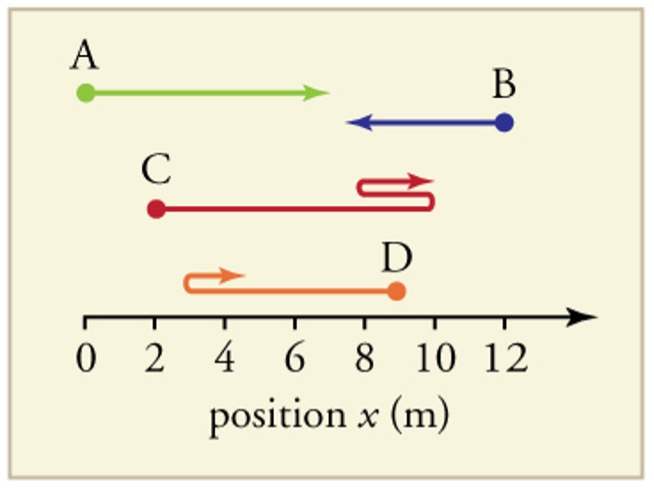
\includegraphics[width=3in]{2-57.jpg}
    \caption{(OpenStax Fig~2.57)}
    \label{2-57}
  \end{figure}

\end{enumerate}\end{multicols}

\vs

\section*{Displacement Conceptual Questions}

Please answer each question in at least one complete sentence

\begin{enumerate}[resume]

  \myquestion (CQ2) 
  Under what circumstances does distance traveled equal magnitude of displacement? %What is the only case in which magnitude of displacement and displacement are exactly the same?
  \vs
  
  \myquestion (CQ3)
  Bacteria move back and forth by using their flagella (structures that look like little tails). Speeds of up to \SI{50}{\micro m/s} (\SI{50e-6}{m/s}) have been observed. The total distance traveled by a bacterium is large for its size, while its displacement is small. Why is this?

  \vs
\end{enumerate}




\pagebreak


\section*{Velocity \& Acceleration Problems}

\begin{multicols}{2}\begin{enumerate}[resume]

\myquestion (P5)  \answer{(a) $\bar{s} \approx \SI{29900}{m/s}$; (b) $\bar{v} = \SI{0}{m/s}$}
(a) Calculate Earth's average speed relative to the Sun (in m/s). (b) What is its average velocity over a period of one year?  (The average radius of the earth's orbit is \SI{1.5e11}{m}.)

\myquestion (Based on Giancolli P2-1)  \answer{60 m}
If you are driving  on the interstate at 30.0~m/s (about 70~MPH) and you look away from the road to check your phone for 2.0~seconds, how far does the car travel during this inattentive period?

\myquestion (P7)  \answer{16.7 million years or \num{5.27e14} seconds}
The North American and European continents are moving apart at a rate of about 3 cm/year. At this rate how long will it take them to drift 500 km farther apart than they are at present?

\myquestion (P16)  \answer{\SI{4.29}{m/s^2}}
A cheetah can accelerate from rest to a speed of 30.0~m/s in 7.00 s. What is its acceleration?


\myquestion (P17)  \answer{(a) $\SI{56.4}{m/s^2}=5.76g$; (b) $\SI{-201}{m/s^2}=20.6g$}
\emph{Professional Application.}
Dr. John Paul Stapp was U.S. Air Force officer who studied the effects of extreme deceleration on the human body. On December 10, 1954, Stapp rode a rocket sled, accelerating from rest to a top speed of 282~m/s (1015~km/h) in 5.00~s, and was brought jarringly back to rest in only 1.40~s! Calculate his (a) acceleration and (b) deceleration. Express each in multiples of $g$ (\SI{9.8}{m/s^2}) by taking its ratio to the acceleration of gravity.




\end{enumerate}\end{multicols}

\pagebreak

\section*{Velocity \& Acceleration Conceptual Questions}

Please answer each question in at least one complete sentence

\begin{enumerate}[resume]

\myquestion (CQ6)
Acceleration is the change in velocity over time. Given this information, is acceleration a vector or a scalar quantity? Explain. \vs

\myquestion (CQ13) 
Is it possible for speed to be constant while acceleration is not zero? Give an example of such a situation. \vs

\myquestion (CQ14) 
Is it possible for velocity to be constant while acceleration is not zero? Explain. \vs

\myquestion (CQ15) 
Give an example in which velocity is zero yet acceleration is not. \vs


\end{enumerate}

\section*{Graphical Analysis Questions}

\begin{enumerate}[resume]

\myquestion (P59, modified) \answer{(a) $v\approx \SI{115}{m/s}$; (b) $a \approx \SI{5.0}{m/s^2}$}
Estimate the (a) velocity and (b) acceleration at $t=20$~s of the jet car whose position is graphed in Figure~\ref{2.59}.

\begin{multicols}{2}

  \begin{figure}[H]
    \centering
    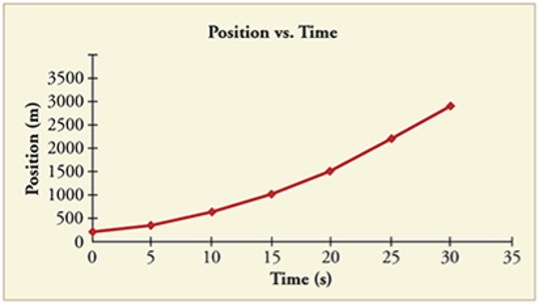
\includegraphics[height=1.7in]{2-58.jpg}
    \caption{(OpenStax Fig~2.58)}
    \label{2.58}
  \end{figure}

  \begin{figure}[H]
    \centering
    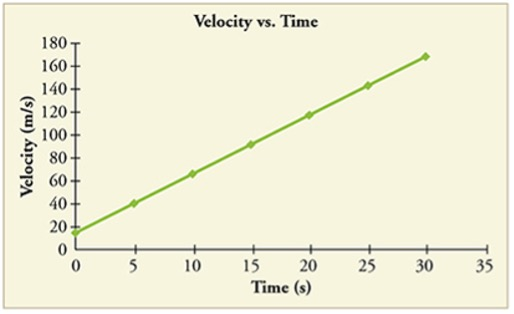
\includegraphics[height=1.7in]{2-59.jpg}
    \caption{(OpenStax Fig~2.59)}
    \label{2.59}
  \end{figure}
  
\end{multicols}
\vs

\pagebreak


\myquestion (P61, modified) \answer{$v\approx\SI{0.25}{m/s}$}
  Estimate the slope of the curve in Figure~\ref{2.60} to find the velocity at $t=30$~s.

  \begin{multicols}{2}

    \begin{figure}[H]
      \centering
      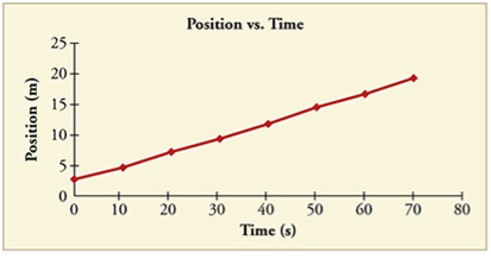
\includegraphics[width=2.8in]{2-60.jpg}
      \caption{(OpenStax Fig~2.60)}
      \label{2.60}
    \end{figure}

    \columnbreak

    \vfill

  \end{multicols}


\myquestion (CQ26, modified) \answer{(a) $t_a$; (b) $t_d$; (c) $t_e$.}
  Consider the graph of position versus time in Figure~\ref{2.52} Identify (a) the time ($t_a$, $t_b$, $t_c$, $t_d$, or $t_e$) at which the instantaneous velocity is greatest, (b) the time at which it is zero, and (c) the time at which it is negative. (d) \emph{Explain your answers}.

  \begin{multicols}{2}
    \begin{figure}[H]
      \centering
      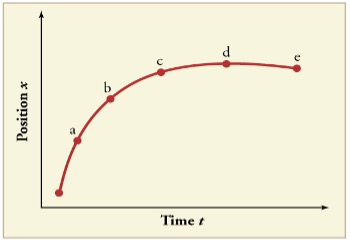
\includegraphics[width=2.8in]{2-52.jpg}
      \caption{(OpenStax Fig~2.52)}
      \label{2.52}
    \end{figure}


    \columnbreak

    \vfill
  

  \end{multicols}


\myquestion (CQ27, modified)
  Sketch a graph of velocity versus time corresponding to the graph of position versus time given in Figure~\ref{2.53}.

  \begin{multicols}{2}

    \begin{figure}[H]
      \centering
      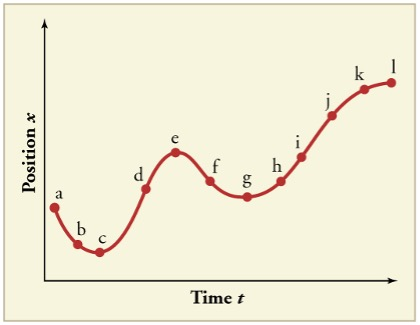
\includegraphics[width=2.8in]{2-53.jpg}
      \caption{(OpenStax Fig~2.53)}
      \label{2.53}
    \end{figure}

    \columnbreak

    \hfill

    \begin{tikzpicture}
      \draw[->] (0,-0.5) -- (0,4.5)
        node[midway, above, sloped] {Velocity $v$};
      \draw[->] (-0.5,0) -- (6,0) 
        node[midway, below] {Time $t$};

    \end{tikzpicture}

  \end{multicols}

\end{enumerate}


\pagebreak

\section*{Additional Practice}
These problems are provided for extra practice.  They are not required and there is no bonus for doing them.

\begin{multicols}{2}


  
\begin{enumerate}[resume]

\myquestion (P9)  \answer{$\SI{34.689}{m/s}=\SI{124.88}{km/h}$}
On May 26, 1934, a streamlined, stainless steel diesel train called the Zephyr set the world's nonstop long-distance speed record for trains. Its run from Denver to Chicago took 13 hours, 4 minutes, 58 seconds, and was witnessed by more than a million people along the route. The total distance traveled was 1633.8 km. What was its average speed in km/h and m/s?

\myquestion (P18)  \answer{(a) \SI{1.43}{s}; (b) \SI{-2.50}{m/s^2}}
A commuter backs her car out of her garage with an acceleration of \SI{1.40}{m/s^2}. (a) How long does it take her to reach a speed of 2.00 m/s? (b) If she then brakes to a stop in 0.800~s, what is her deceleration?


\myquestion (CQ28)
(a) Explain how you can determine the acceleration over time from a velocity versus time graph such as the one in Figure~\ref{2.54}. (b) Based on the graph, how does acceleration change over time?

    \begin{figure}[H]
      \centering
      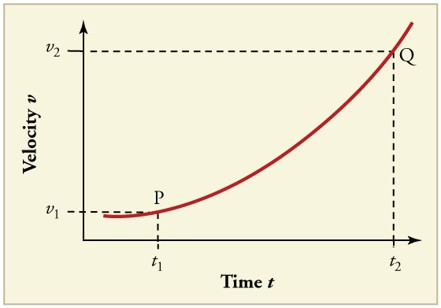
\includegraphics[width=2.8in]{2-54.jpg}
      \caption{(OpenStax Fig~2.54)}
      \label{2.54}
    \end{figure}


\myquestion (CQ29) \answer{(b) $t=t_b$ \& $t\ge t_j$; (c) $t_d$ \& $t_h$; $t>t_h$}
(a) Sketch a graph of acceleration versus time corresponding to the graph of velocity versus time given in Figure~\ref{2.55}. (b) Identify the time or times ($t_a$, $t_b$, $t_c$, etc.) at which the acceleration is greatest. (c) At which times is it zero? (d) At which times is it negative?

    \begin{figure}[H]
      \centering
      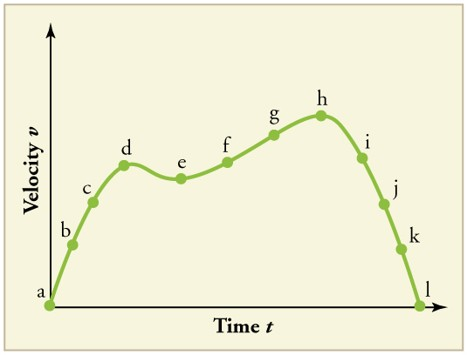
\includegraphics[width=2.8in]{2-55.jpg}
      \caption{(OpenStax Fig~2.55)}
      \label{2.55}
    \end{figure}

\end{enumerate}



% \section*{Bonus}

% You will be given bonus if you complete these problems \emph{on a separate sheet of paper}
  
% \begin{enumerate}[resume]


% \myquestion  
  
% \end{enumerate}
\end{multicols}



\end{document}